
\section{Problem statement}
In this section we provide the context in which this current work has been performed. Our objective in this work is to develop a fast technique to classify current laser data into static and dynamic parts. This work will be used in the framework of Bayesian Occupancy Filter (BOF)\cite{coue:inria-00182004, mekhnacha:inria-00336356} to accomplish some reduction in processing time. Inorder to understand the relevance of this work we first need to understand how BOF works. In the following we first summarize the working of BOF framework and then state the context of the problem addressed in this work.
\subsection{Bayesian Occupancy Filter (BOF)}
In this section we summarize the working of BOF detailed in \cite{mekhnacha:inria-00336356}. The Bayesian Occupancy Filter (BOF) is represented as a two dimensional planar grid based decomposition of the environment. Each cell of the grid contains two probability distributions. A probability distribution on the occupancy of the cell, and the probability distribution on the velocity of the cell occupancy.

Given a set of input sensor readings, the BOF algorithm allows to update the occupancy/velocity estimates of each grid cell. Since BOF is a filtering technique so it, essentially, is based on prediction and estimation (updating) steps as shown in figure \ref{fig:bf}. The key idea of the model is to represent the 2D space using a regular grid. Given this space discretization and assuming that objects do not overlap, the velocity of a given cell $c$ at a time $t$ is directly linked to the identity of its antecedent cell $A^c$ from which the content of cell $c$ moved between $t-1$ and $t$. In other words, we can define the velocity of a given cell by providing the index of its antecedent (previous position).

\begin{figure}[H]
   \centering
     \begin{tabular}{lr}
       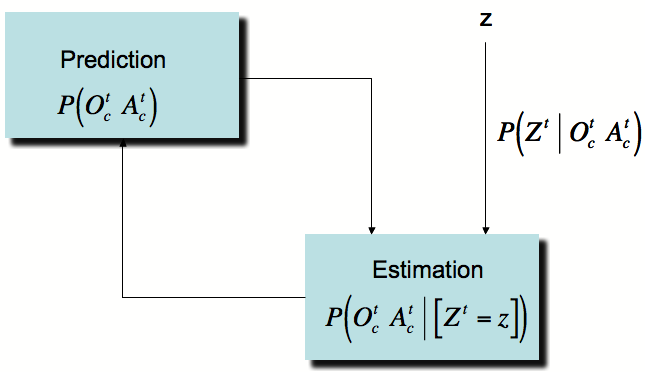
\includegraphics[scale=0.5]{img/fig:bf}
     \end{tabular}
   \caption{BOF prediction and estimation cycle}
   \label{fig:bf}
\end{figure}

Therefore, estimating the velocity of a given cell is equivalent to estimating a probability table over its all possible antecedents. Possible antecedents of a cell are defined by providing a neighborhood from which the cell is reachable in a time step.

Formally if $A_t^c$ represents each antecedent of cell $c$ at time $t$, $A_{t-1}^c$ gives all antecedents of the same cell at time $t-1$, $O_t^c=\{0,1\}$ specifies if cell is empty or occupied and $Z_t$ represents current sensor reading, then BOF estimates the following posterior joint probability:
\begin{equation}
P(A_{t-1}^c A_t^c O_t^c Z_t) = P(A_{t-1}^c)P(A_t^c|A_{t-1}^c)P(O_t^c|A_{t-1})P(Z_t|A_t^c,O_t^c)
\end{equation}

It is important to note that velocity estimates are done without any motion sensor information, however this approach has two important limitations:
\begin{enumerate}
\item We must define an effective velocity range and this range must be discretized with appropriate resolution.
\item We must specify a neighborhood size where the antecedents search will take place.
\end{enumerate}
These two limitations have some consequences, objects moving with velocities beyond this range will not be detected. This range cannot be taken large otherwise discretization will result in long array of velocity values that must be processed for each cell during BOF cycle, increasing processing time. Similarly neighborhood size can also create a limitation. A small neighborhood size mean fast calculations but cells moving more than that size, during $t-1$ to $t$, will not be detected. Whereas a big neighborhood size means more processing time, since calculations will be done for each cell in the neighborhood. This leads us to the following hypothesis.

\subsection{Report Hypothesis}
Given the above limitations we hypothesize that if vehicle motion information are available then we can use them to do a fast distinction between static and dynamic parts of the environment. This distinction can help us restrict the search and calculations in the BOF framework to only those regions where motion has been detected. Since, normally most of the part of the environment is static so this will allow us to decrease the calculation time greatly and will allow us to have increased velocity range and bigger neighborhood size around the moving parts. These improvements will result in better results.

Since this is a master internship work so during this time we will only be developing technique to do a fast distinction between static and dynamic parts of the environment. However its integration with BOF framework will be left as future work.

\section{State of the art}
%%%%%%%%%%%%%%%%%%%%%%%%%%%%%%
In this section we are going to introduce the current state of the research conducted in the robotics perception, specifically for classification between static and dynamic objects/parts. Some of the methods presented in this section follow similar goals as ours, but due to different applicability and/or constraints, it was necessary to develop the new method presented in this document to fill up our needs.

To present 3rd parties work, we are going to follow a same guide. First introduce their real goal, then the solution without the intrinsic technical the details. For the closure a discussion about their results and why their method was not suitable for our application.

\section{Tackling the problem}

There have been several proposals toward a good classification methods, all on behalf of scene understanding. Due to the variety of sensors and problem to tackle the techniques can vary. Thus, techniques may have to be adapted according to the issue and the situation that the method is applied.

The work over this theme copes with task of understanding the environment by knowing the objects that are present. For that reason, being able to distinguish the objects in the environment is important. Depending on the granularity of the distinction performed by the method authors can name it differently, like: separation, segmentation, classification, identification, etc. \cite{Wolf04onlinesimultaneous} \cite{DBLP:conf/iros/LidorisWB08} are some examples of researches conducted with the intent to separate the dynamic and static environments.

\section{Grouping processes in robotics}

One important step in the scene understanding is the environment map building and the localization of the ego-robot inside this map. This problem is known as SLAM \cite{Leonard2002Mobile} \cite{qadeerthesis}, which stands for Simultaneous Localization and  Mapping.

SLAM is composed of several steps to achieve its goals: landmark extraction, data association, state estimation are some examples. Each of them can be solved using different techniques.

SLAM assumes static environment constraint, in another words, assumes that there are no moving objects in the same environment as the robot. Moving objects would interfere negatively in the mapping process. For this reason, there is another process called DATMO to deal with the dynamism of the environment.

DATMO stands for Detection and Tracking of Moving Objects. When dealing with mobile robots in a dynamic environment we apply the DATMO process to obtain the moving objects from the environment.

Several researchers have been dedicated to solve the SLAM problem in dynamic environments, sometimes called SLAMIDE\cite{bibbyrss07}. Other alternatives like solving SLAM with DATMO\cite{Wang02simultaneouslocalization} emerged as well.

\section{Approaches for motion detection}

\subsection{Stereo-vision camera}

In the Henning Lategahn and Bernd Kitt work \cite{DBLP:conf/ivs/LategahnGHKE11}, they proposed a method to separate the static and dynamic environment using stereo-vision camera. Their method uses a probabilistic approach of classification. Due to the probabilistic technique that was choose, this approach is not well suited for our purpose, which is to distinguish those two groups using the minimum amount of time.

Their work was evaluated theoretically and concretely. The theoretical test done by simulation and the final test done in a real footage from a moving vehicle.

The results were promising, although in some situations the correct separation was given only after processing 19 samples of the environment. 

Although we have the same goal, we applied different constraints and acceptance conditions for the application. 

\subsection{Mono-vision camera}

In the work developed by Migliore et al. \cite{Migliore_2009_ICRA} is a MONOSLAM process (SLAM applied with no IMU data, and mono-vision camera), this method uses feature detector algorithms, named Shadow Filter, to provided anchors in the image. Those anchors established during while the robot is moving, they work as dynamic landmarks. The algorithms make use of them to solve the SLAM.

Their method uses as input the initial position of the camera information and a mono-vision camera as sensor to perceive the environment. This configuration is not reliable for to solve our problem due to the number of assumptions and filters applied to the mono-vision camera to obtain the feature.

This method was tested in a non-crowded environment and has shown its applicability, but due to bad performance with small displacements is not suited for the ADAS system, which acquire several frames in one second, in which the displacement is fairly small. Beyond that, our approach is focused in laser scanner as sensor to perceive the environment.

\subsection{LIDAR approach}

In the work \cite{4650636}, they were able to classify the objects in the scene by a larger chain of processes to solve some issues with the data acquired. This method the relies on several steps to correct/fuse the laser data readings, among these processes there is scan segmentation(Euler distance), scan alignment(Iterative Closest Point \cite{10.1109/34.121791}) before perform the motion detection itself. 

%In our   was used to establish the displacement of the objects in the scene. 

In our method, we use as input an occupancy grid, in which the scan alignment is not needed, since the occupancy grid gives us a fusion view of the laser scanner reading. Besides, the clustering could be done in the occupancy grid, but would not be coherent with our final goal of knowing the dynamic and static parts of the environment.


